\documentclass{beamer}
\usetheme{Copenhagen}
\usepackage{xeCJK}
\setCJKmainfont{Noto Serif CJK SC}
 
 
%Information to be included in the title page:
\title{多线程并行 InSAR 数据处理\\程序的设计与实现}
\author{崔灏 PB13007103}
\institute{中国科学技术大学\\地球和空间科学学院}
\date{\today}
 
 
\begin{document}

\frame{\titlepage}

\begin{frame}
    \frametitle{课题介绍}
    \framesubtitle{背景}

    \textbf{合成孔径雷达干涉成像(InSAR)}技术:
    \begin{itemize}
        \item 两幅 SAR 干涉成像:相位差 $\to$ 高程/形变(厘米级)
        \item 大地测量的重要手段
    \end{itemize}

    数据处理:
    \begin{itemize}
        \item SAR 数据量大(ALOS: 1.2GB/frame,数百 km 范围)
        \item InSAR 数据处理算法复杂
        \item 软件:GMTSAR(开源/免费)、ISCE(需要申请)
    \end{itemize}
\end{frame}


\begin{frame}
    \frametitle{课题介绍}
    \framesubtitle{动机}

    普通研究人员(我们):
    \begin{itemize}
        \item 桌面电脑处理数据
        \item 软件串行处理,CPU 主频有限
        \item 完整流程等待 20min~hours
    \end{itemize}

    CPU 硬件发展:
    \begin{itemize}
        \item 主频达到瓶颈($<$4GHz)
        \item 多核心 CPU 普及 $\to$ 并行计算能力提升
    \end{itemize}

    要使用多核心 CPU 加速 InSAR 数据处理,必须将算法\textbf{并行化}。
\end{frame}

\begin{frame}
    \frametitle{课题介绍}
    \framesubtitle{成果}

    本课题:
    \begin{itemize}
        \item 以 GMTSAR 开源代码(串行算法)为范本
        \item 选取 InSAR 数据处理中两个模块,重写为并行程序:
        \begin{itemize}
            \item 图像配准(image registration)
            \item 图像拼接(image stitching)
        \end{itemize}
        \item 在实际 SAR 数据上测试了新程序,证明并行算法:
        \begin{itemize}
            \item 没有降低算法精度
            \item 大大提高了 InSAR 数据处理效率
        \end{itemize}
    \end{itemize}
\end{frame}

\begin{frame}
    \frametitle{算法设计}
    \framesubtitle{InSAR 基础}


    \begin{columns}
        \begin{column}{0.5\textwidth}
            \centering

            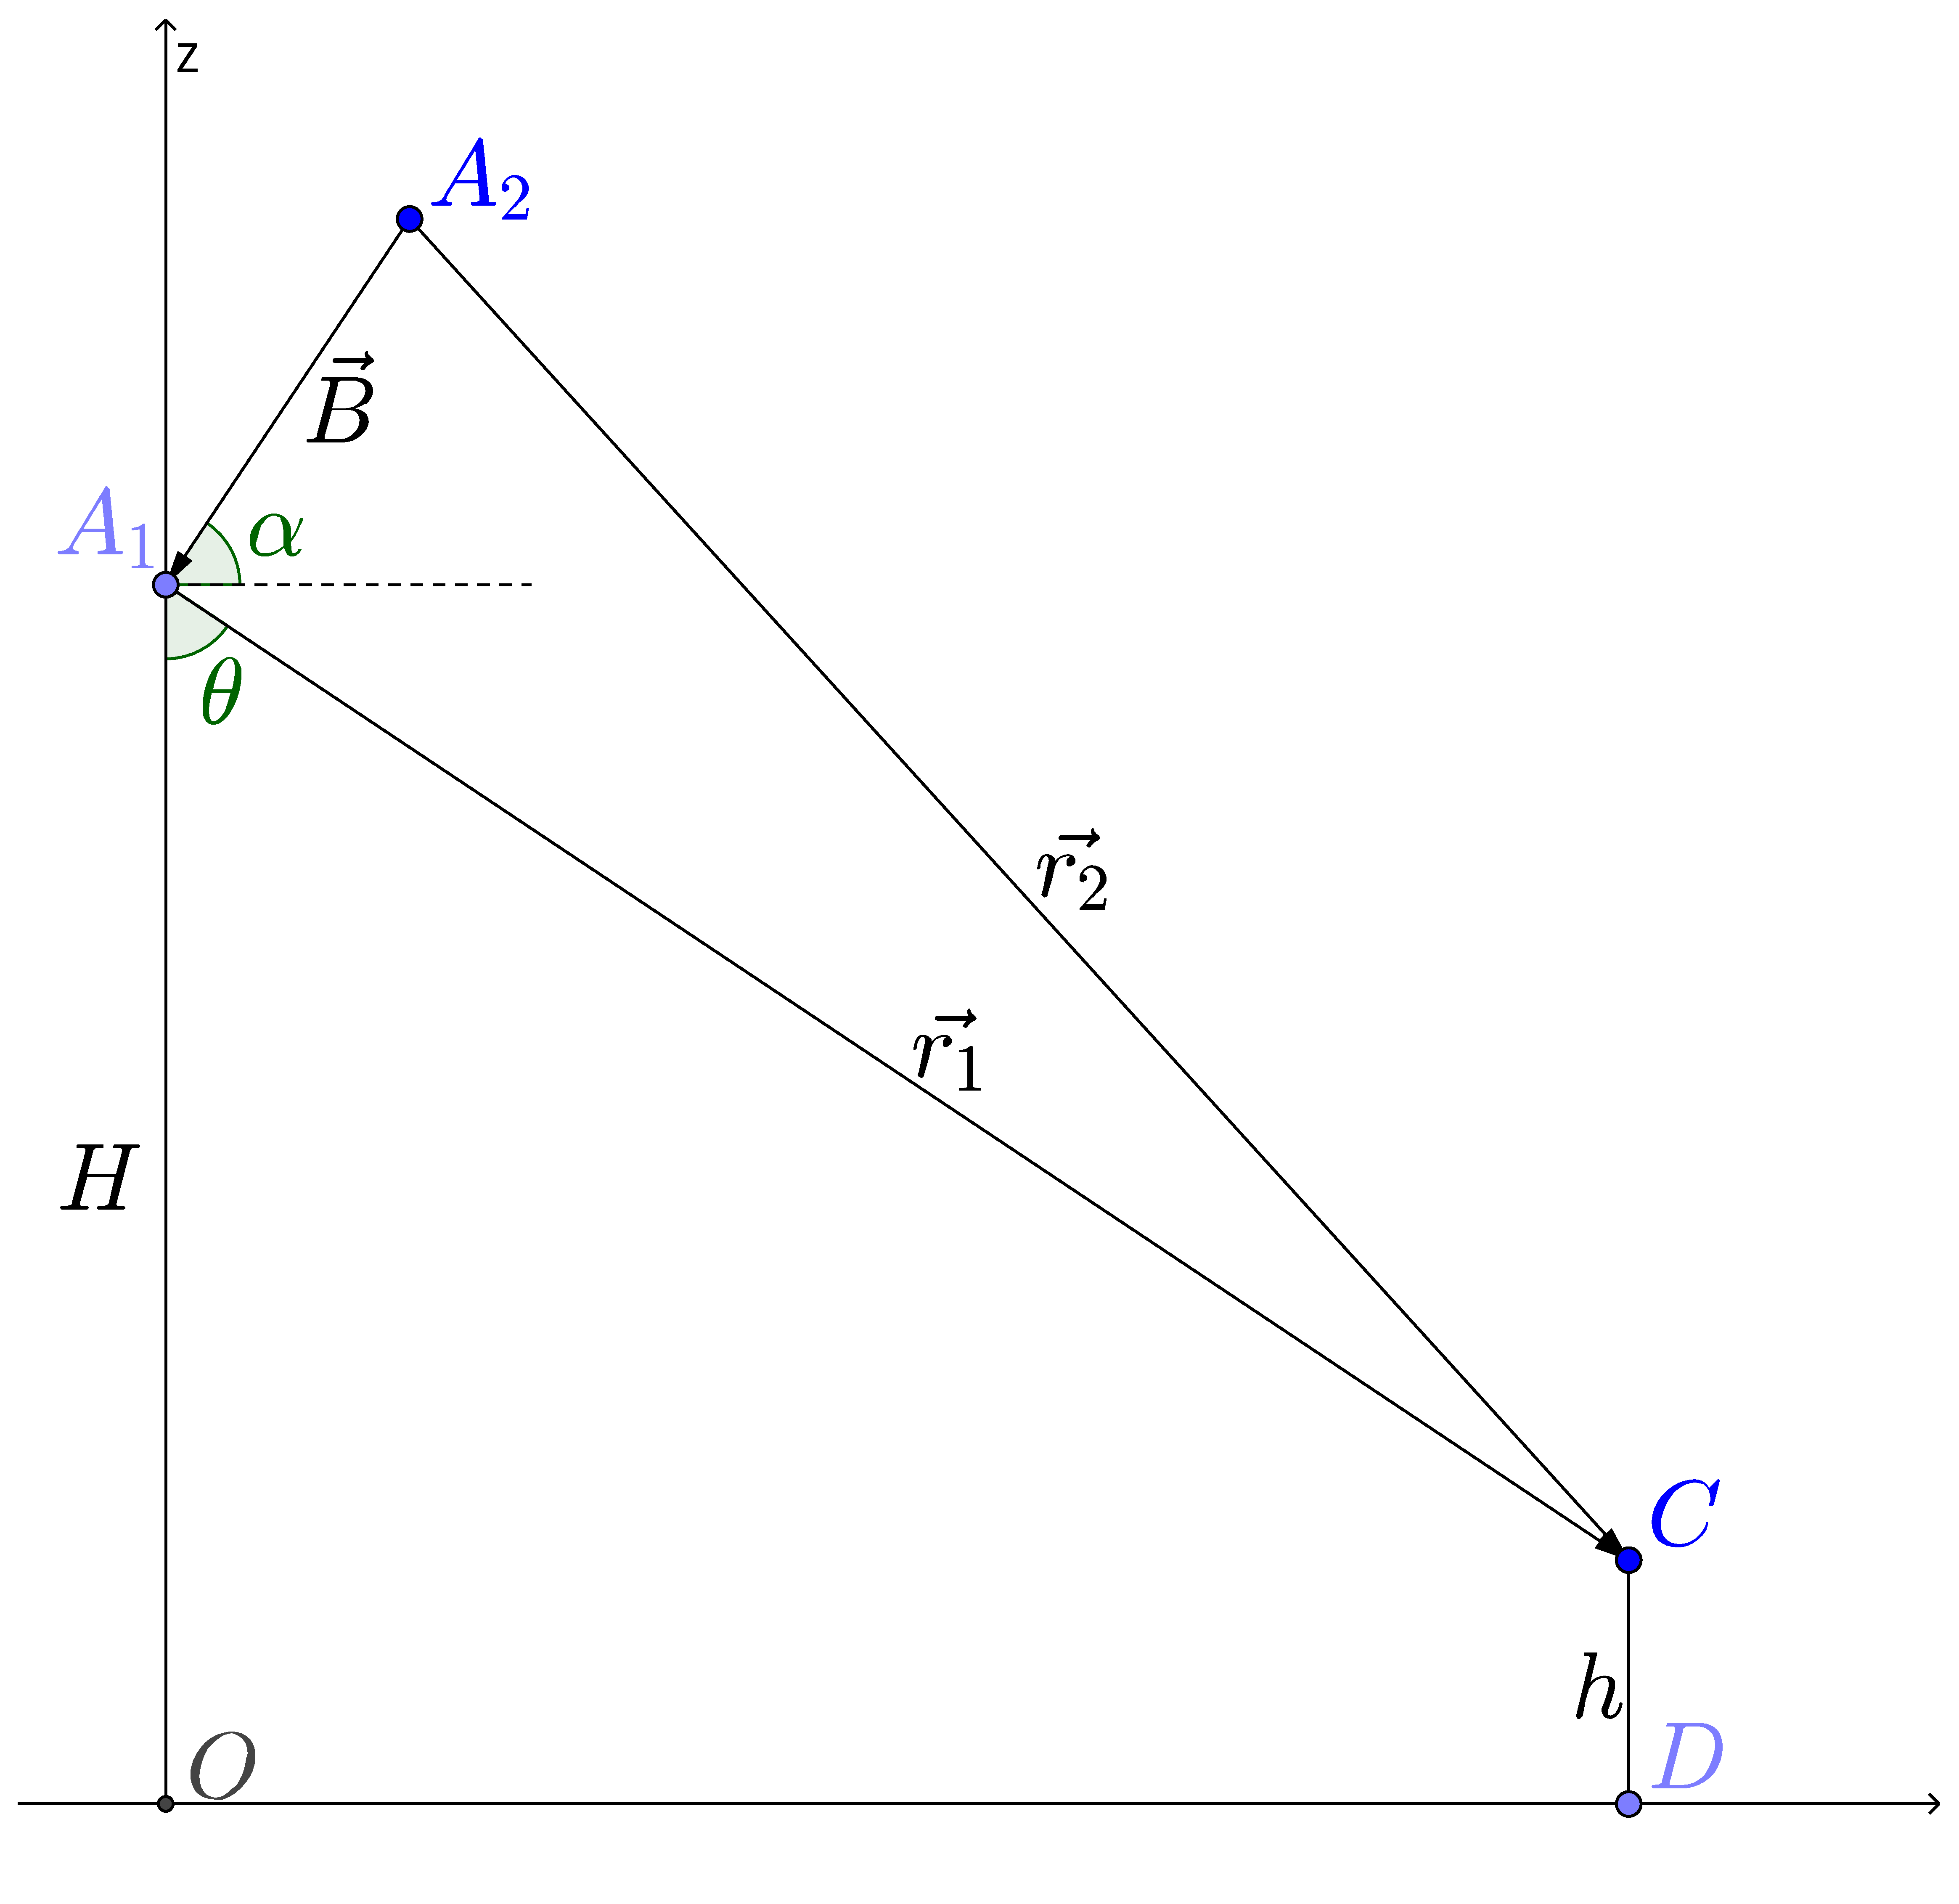
\includegraphics[width=0.8\textwidth]{figures/insar_simple.pdf}

            \resizebox{0.8\textwidth} {!} {
                \begin{minipage}{\linewidth}
                \begin{align*}
                    h &= H - r_1 \cos\theta \\
                    P_{\textrm{干涉}} &= P_1^* P_2 =  A_1 A_2 \exp(i \frac{4\pi}{\lambda}(r_2 - r_1)) \\
                    r_2 - r_1 &= r_1 \sqrt{1- \frac{\vec{r_1} \cdot \vec{B}}{r_1} + (\frac{B}{r_1})^2} \\
                              &\approx - \vec{r_1} \cdot \vec{B} \qquad \because B \ll |\vec{r}| \\
                              &= - r_1 B \cos(\frac{\pi}{2} - \theta + \alpha)
                \end{align*}
                \end{minipage}
            }
        \end{column}
        \begin{column}{0.5\textwidth}
            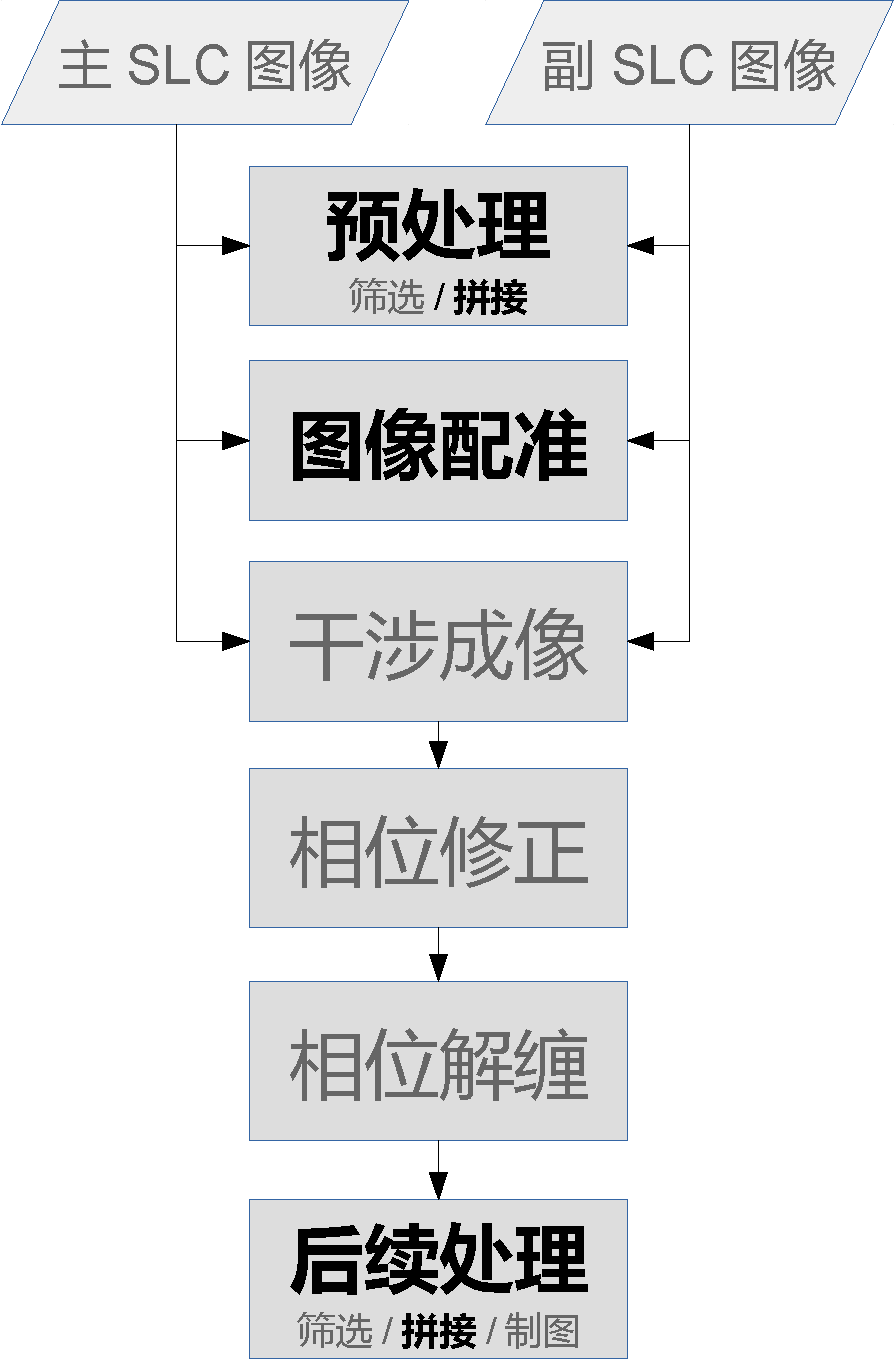
\includegraphics[width=0.9\textwidth]{figures/process.pdf}
        \end{column}
    \end{columns}
\end{frame}


\begin{frame}
    \frametitle{算法设计}
    \framesubtitle{图像配准:GMTSAR xcorr}

    \begin{columns}
        \begin{column}{0.5\textwidth}
            \footnotesize
            \begin{center}
                图像配准 $(x_i, y_i) \to (x'_i, y'_i)$:
                \begin{equation*}
                    \begin{bmatrix}
                        t_i x_i' \\
                        t_i y_i' \\
                        t_i \\
                    \end{bmatrix}
                    = \begin{bmatrix}
                        a & b & c \\
                        d & e & f \\
                        0 & 0 & 1 \\
                    \end{bmatrix}
                    \begin{bmatrix}
                        x \\
                        y \\
                        1 \\
                    \end{bmatrix}
                \end{equation*}
                采样 $\to$ 局部配准 $\to$ 拟合全局参数\\
                要求精度:1/10 像素
            \end{center}

            局部配准:
            \begin{itemize}
                \item 粗配准(天线参数)+精配准\\
                \item \tiny $ (x'_c, y'_c)_{i,j} = (x_c, y_c)_{i,j} + (\Delta_x, \Delta_y) + (\delta_x, \delta_y)_{i,j} $
            \end{itemize}
        \end{column}
        \begin{column}{0.5\textwidth}
            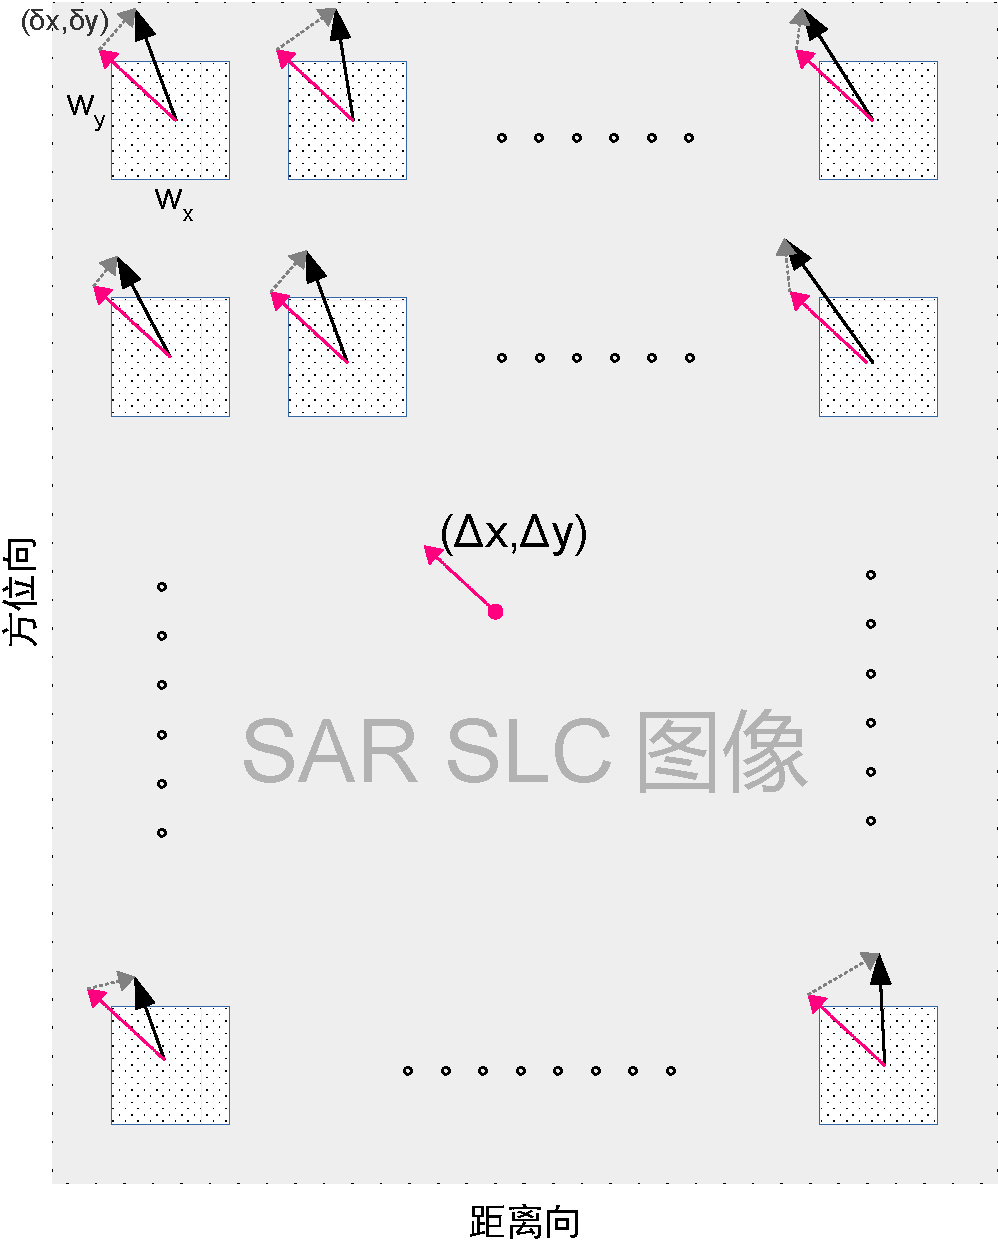
\includegraphics[width=0.80\textwidth]{figures/register.pdf}
        \end{column}
    \end{columns}

    \centering
    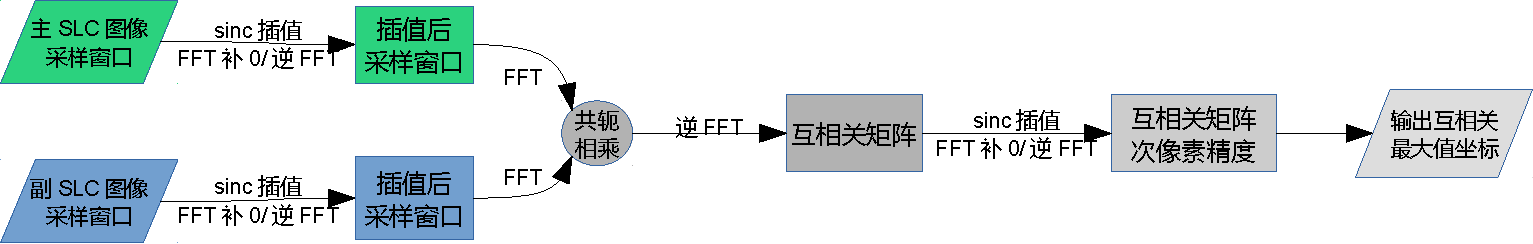
\includegraphics[width=0.99\textwidth]{figures/xcorr-crop.pdf}
\end{frame}

\begin{frame}
    \frametitle{算法设计}
    \framesubtitle{图像配准优化:xcorr2}

    \begin{block}{简化 FFT}
        局部配准只用到复像素的幅值(散射系数幅度):
        \begin{itemize}
            \item GMTSAR xcorr:9 次 FFT(或逆变换)
            \item xcorr2:4 次 FFT + 5 次实序列 FFT
        \end{itemize}
        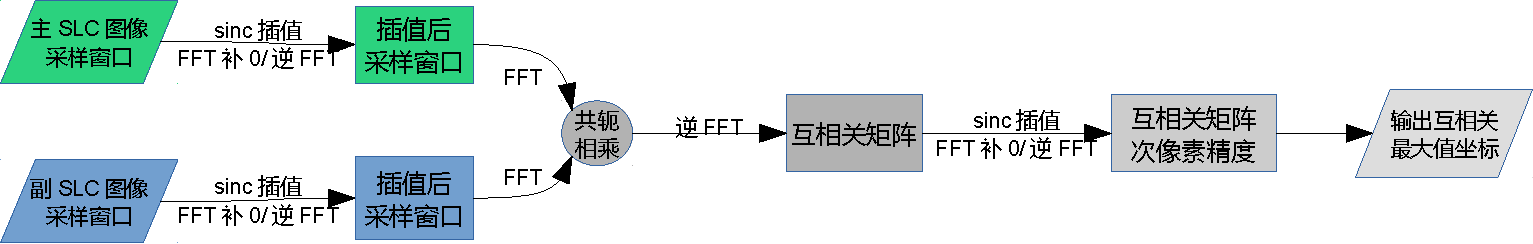
\includegraphics[width=0.99\textwidth]{figures/xcorr-crop.pdf}
    \end{block}
\end{frame}



\begin{frame}
    \frametitle{算法设计}
    \framesubtitle{图像配准优化:xcorr2}

    \begin{columns}
        \begin{column}{0.5\textwidth}
            \begin{block}{主-副多线程架构}
            \begin{itemize}
                \item 主线程加载采样窗口图像
                \begin{itemize}
                    \item 预读取
                    \item 启动计算线程
                \end{itemize}
                \item 计算线程执行局部配准
            \end{itemize}
            \end{block}

            \begin{block}{特点}
            \begin{itemize}
                \item 任务分割粒度小 \\ \begin{scriptsize} 512 采样窗口 vs 4~16 核心 \end{scriptsize}
                \item 数据量大,避免竞争 IO \\ \begin{scriptsize} 磁盘顺序读写优势 \end{scriptsize}
            \end{itemize}
            \end{block}
        \end{column}
        \begin{column}{0.5\textwidth}
            \centering
            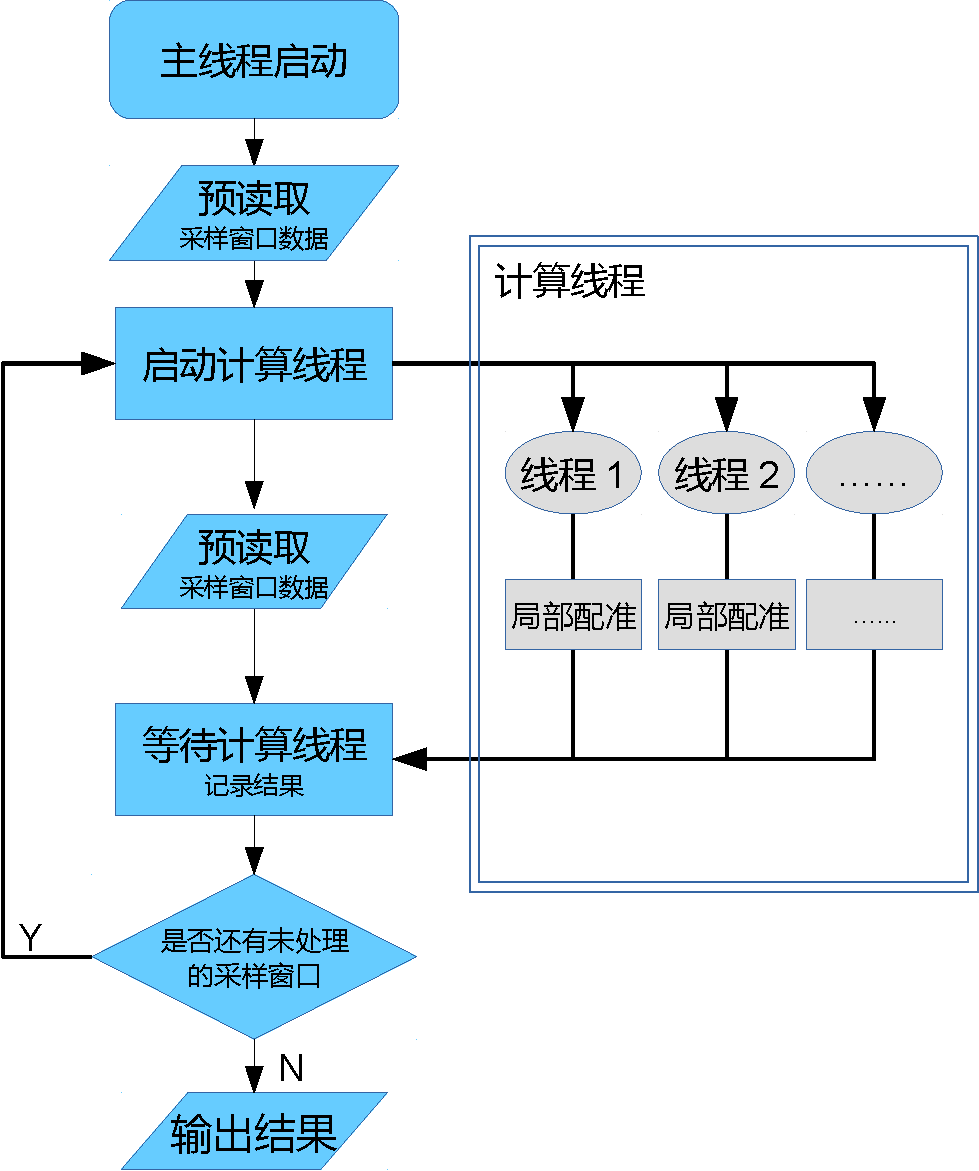
\includegraphics[width=0.99\textwidth]{figures/parallel.pdf}
        \end{column}
    \end{columns}
\end{frame}



\begin{frame}
    \frametitle{算法设计}
    \framesubtitle{图像拼接}

    \begin{columns}
        \begin{column}{0.5\textwidth}
            wowowo
        \end{column}
        \begin{column}{0.5\textwidth}
            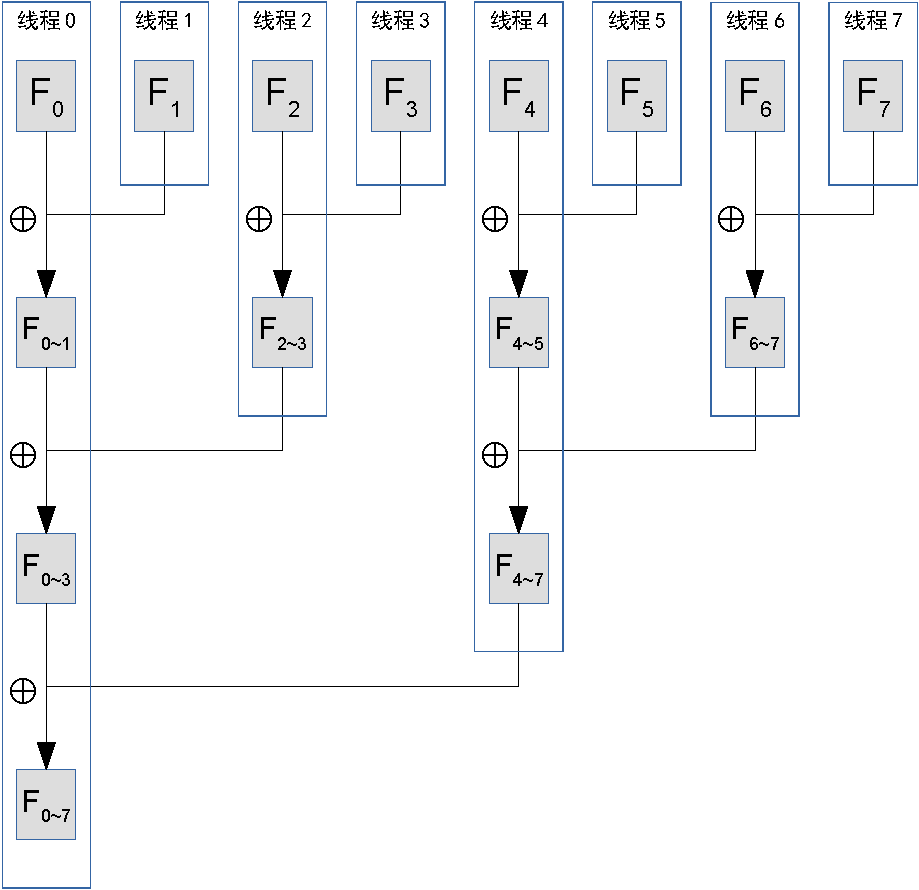
\includegraphics[width=0.99\textwidth]{figures/reduce.pdf}
        \end{column}
    \end{columns}
\end{frame}



\end{document}
